% !TEX root = mth727_lecture_notes.tex


\chapter[Weak Equivalences]{Weak Equivalences}
\chaptermark{Weak Equivalences}
\label{WEAK EQUIVALENCES CHAPTER}
\thispagestyle{firststyle}





\begin{definition}
Let $0 \leq n \leq \infty$. 
A map $f\colon X \to Y$ is an \emph{$n$-equivalence} if the induced homomorphism
$f_{\ast}\colon \pi_{i}(X, x_{0}) \to \pi_{i}(Y, f(x_{0}))$ is an 
isomorphism for  $0\leq i<n$ and it is an epimorphism for $i=n$ for all 
$x_{0}\in X$. A map $f$ is a \emph{weak (homotopy) equivalence} if it is an $\infty$-equivalence.
\end{definition}

Recall that for a map $f\colon X\to Y$ the mapping cylinder of $f$ is the space
\[
M_{f} = (X \times [0, 1] \sqcup Y) / {\sim}
\]
where $(x, 0) \sim f(x)$ for all $x\in X$. We will consider $X$ as a subspace 
of $M_{f}$ by identifying it with $X\times \{1\}$. 

\begin{proposition}
\label{N EQUIV EQUIVAKENT COND PROP}
Given a map $f\colon X \to Y$ the following conditions are equivalent:
\benu
\item[1)] $f$ is an $n$-equivalence.
\item[2)] For $k\leq n$, given any commutative diagram 
\begin{equation*}
\begin{tikzpicture}
\matrix (m) 
[matrix of math nodes, row sep=3em, column sep=3em, text height=1.5ex, text depth=0.25ex]
{
S^{k-1} & X \\
D^{k} &  Y \\
};
\path[->, thick, font=\scriptsize]
(m-1-2) 
edge node[anchor = west] {$f$} (m-2-2)
(m-1-1) 
edge node[above] {$\varphi$} (m-1-2)
(m-2-1) 
edge node[below] {$\psi$} (m-2-2)
;
\path[right hook-latex, thick, font=\scriptsize]
(m-1-1) 
edge
(m-2-1);
\path[dashed, ->,  thick, font=\scriptsize]
(m-2-1) 
edge node[anchor=south east] {$\xov{\psi}$} (m-1-2);
\end{tikzpicture}
\end{equation*}
there exists a map $\xov{\psi}\colon D^{k} \to Y$ 
such that $\xov{\psi}|_{S^{k-1}} = \varphi$ and 
$f \xov{\psi}\simeq \psi \ (\rel S^{k-1})$.

\item[3)] For $k\leq n$, given any diagram 
\begin{equation*}
\begin{tikzpicture}
\matrix (m) 
[matrix of math nodes, row sep=3em, column sep=3em, text height=1.5ex, text depth=0.25ex]
{
S^{k-1} & X \\
D^{k} &  Y \\
};
\path[->, thick, font=\scriptsize]
(m-1-2) 
edge node[anchor = west] {$f$} (m-2-2)
(m-1-1) 
edge node[above] {$\varphi$} (m-1-2)
(m-2-1) 
edge node[below] {$\psi$} (m-2-2)
;
\path[right hook-latex, thick, font=\scriptsize]
(m-1-1) 
edge
(m-2-1);
\path[dashed, ->,  thick, font=\scriptsize]
(m-2-1) 
edge node[anchor=south east] {$\xov{\psi}$} (m-1-2);
\end{tikzpicture}
\end{equation*}
and a homotopy $\Phi\colon f\varphi \simeq \psi|_{S^{k-1}}$
there exists a map $\xov{\psi}\colon D^{k} \to Y$ and a homotopy 
$\xov{\Phi}\colon f\xov{\psi} \simeq \psi$
such that $\xov{\psi}|_{S^{n-1}} = \varphi$
and $\xov{\Phi}|_{S^{k-1}\times [0, 1]} = \Phi$.

\item[4)] The pair $(M_{f}, X)$ is $n$-connected.
\eenu
\end{proposition}

\begin{proof}
Exercise.
\end{proof}




\begin{proposition}
\label{WE PROPERTIES PROP}
1) If $f, g\colon X\to Y$ are maps such that $f\simeq g$ and $f$ is 
an $n$-equivalence then so is $g$. 

2) If $f\colon X\to Y$, $g\colon Y \to Z$, and any two of the maps $f$, $g$, $gf$
are weak equivalences, then so is the third map. 

3) Every homotopy equivalence is a weak equivalence. 
\end{proposition}

\begin{proof}
Exercise.
\end{proof}




One of the main goals of this chapter will be the proof of the following fact: 

\begin{theorem}
\label{WEAK EQUIV CW THM}
If $X$, $Y$ are CW complexes then any weak equivalence $f\colon X\to Y$ is a homotopy 
equivalence.
\end{theorem}


\begin{note}
Theorem \ref{WEAK EQUIV CW THM} does not hold in general for spaces that are not 
CW complexes. For example, let $W$ be the Warsaw circle (shown below). Since 
$\pi_{i}(W) = 0$ for all $i$, the constant map $W \to \ast$ is a weak equivalence.  
However, it is not a homotopy equivalence.

\begin{equation*}
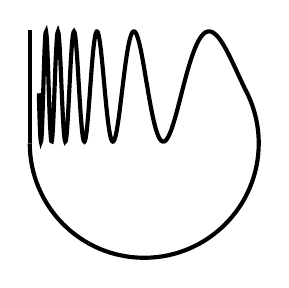
\begin{tikzpicture}[scale =0.7] 
\draw[line width = 1.5] (2.1, -1.03) -- (2.1, 1.03);
\begin{scope}
\draw[xscale=15, line width = 1.5 , domain= 0.151:0.40123,smooth,variable=\x, samples = 400] plot ({\x},{sin(pow(\x, -2) r)});
\end{scope}
\draw[line width = 1.5] (2.1, -1.03) arc [radius = 2.0772, start angle = 180, end angle = 388.15];

\end{tikzpicture}
\end{equation*}
\end{note}


The proof Theorem \ref{WEAK EQUIV CW THM} will use the following fact:


\begin{proposition}
\label{HELP PROP}
Assume that we have a diagram 
\begin{equation*}
\begin{tikzpicture}
\matrix (m) 
[matrix of math nodes, row sep=3em, column sep=3em, text height=1.5ex, text depth=0.25ex]
{
A & Y \\
X &  Z \\
};
\path[->, thick, font=\scriptsize]
(m-1-2) 
edge node[anchor = west] {$f$} (m-2-2)
(m-1-1) 
edge node[above] {$g$} (m-1-2)
(m-2-1) 
edge node[below] {$h$} (m-2-2)
;
\path[right hook-latex, thick, font=\scriptsize]
(m-1-1) 
edge
(m-2-1);
\path[dashed, ->,  thick, font=\scriptsize]
(m-2-1) 
edge node[anchor=south east] {$\xov{h}$} (m-1-2);
\end{tikzpicture}
\end{equation*}
where $(X, A)$ is a relative CW complex such that $\dim(X\setminus A) \leq n$ for 
some $n\leq \infty$, and $f\colon Y \to Z$ is an $n$-equivalence.
Assume also that $\Phi\colon A\times [0, 1] \to Z$ is a homotopy such that 
$\Phi\colon h|_{A} \simeq gf$. Then there exists a map $\xov{h}\colon X \to Y$
and a homotopy $\xov{\Phi}\colon X\times [0, 1] \to Z$ such that $\xov{h}|_{A} = g$, 
$\xov{\Phi}\colon h \simeq f\xov{h}$ and 
$\xov{\Phi}|_{A\times [0, 1]} = \Phi$. 
\end{proposition}

\begin{proof}
By induction on skeleta of $(X, A)$, using 
Proposition \ref{N EQUIV EQUIVAKENT COND PROP}.
\end{proof}

As a special case of Proposition \ref{HELP PROP} we obtain:

\begin{corollary}
\label{HELP COR}
Assume that we have a commutative diagram 
\begin{equation*}
\begin{tikzpicture}
\matrix (m) 
[matrix of math nodes, row sep=3em, column sep=3em, text height=1.5ex, text depth=0.25ex]
{
A & Y \\
X &  Z \\
};
\path[->, thick, font=\scriptsize]
(m-1-2) 
edge node[anchor = west] {$f$} (m-2-2)
(m-1-1) 
edge node[above] {$g$} (m-1-2)
(m-2-1) 
edge node[below] {$h$} (m-2-2)
;
\path[right hook-latex, thick, font=\scriptsize]
(m-1-1) 
edge
(m-2-1);
\path[dashed, ->,  thick, font=\scriptsize]
(m-2-1) 
edge node[anchor=south east] {$\xov{h}$} (m-1-2);
\end{tikzpicture}
\end{equation*}
where $(X, A)$ be a relative CW complex such that $\dim(X\setminus A) \leq n$ for 
some $n\leq \infty$, and $f\colon Y \to Z$ is an $n$-equivalence.
Then there exists a map $\xov{h}\colon X\to Y$ such that $\xov{h}|_{A} = g$
and $f\xov{h} \simeq h \ (\rel A)$.
\end{corollary}



Recall that by $[X, Y]$ we denote the set of homotopy classes of maps $X \to Y$. 
A map $f\colon Y\to Z$ induces a map of sets $f_{\ast} \colon [X, Y]\to [X, Z]$
given by $f_{\ast}[\varphi] = [f\varphi]$. 

\begin{corollary}
\label{N EQUIV HOMOT CLASSES COR}
Let $f\colon Y \to Z$ be an $n$-equivalence for some $n\leq \infty$. 
For any CW complex $X$ the map 
\[
f_{\ast} \colon [X, Y] \to [X, Z]
\]
is a bijection if $\dim X \leq n - 1$ and it is onto if $\dim X \leq n$. 
\end{corollary}

\begin{proof}
The onto part follows from Corollary \ref{HELP COR} with $A=\varnothing$. 
It remains to show that $f_{\ast}$ is 1-1 if $\dim X \leq n-1$. Assume then 
that for some $\varphi_{0}, \varphi_{1}\colon X \to Y$ there is a homotopy 
$h\colon X \times [0, 1] \to Z$ such that $h_{0} = f\varphi_{0}$ and 
$h_{1} = f\varphi_{1}$. This gives a commutative diagram
\begin{equation*}
\begin{tikzpicture}
\matrix (m) 
[matrix of math nodes, row sep=3em, column sep=3em, text height=1.5ex, text depth=0.25ex]
{
X\times \{0, 1\} & Y \\
X\times [0, 1] &  Z \\
};
\path[->, thick, font=\scriptsize]
(m-1-2) 
edge node[anchor = west] {$f$} (m-2-2)
(m-1-1) 
edge node[above] {$\varphi_{0}\sqcup \varphi_{1}$} (m-1-2)
(m-2-1) 
edge node[below] {$h$} (m-2-2)
;
\path[right hook-latex, thick, font=\scriptsize]
(m-1-1) 
edge  node[anchor = east] {$i$}
(m-2-1);
\path[dashed, ->,  thick, font=\scriptsize]
(m-2-1) 
edge node[anchor=south east] {$\xov{h}$} (m-1-2);
\end{tikzpicture}
\end{equation*}

Consider the relative CW complex 
$(X \times [0, 1], X\times \{0, 1\})$. Since $\dim X\times [0, 1] \leq n$, 
using Corollary \ref{HELP COR}
again we obtain that there exists $\xov{h}\colon X\times [0, 1] \to Y$ which is homotopy 
between $\varphi_{0}$ and  $\varphi_{1}$. 
\end{proof}


\begin{proof}[Proof of Theorem \ref{WEAK EQUIV CW THM}]
Let $f\colon X \to Y$ be a weak equivalence of CW complexes. 
By Corollary \ref{N EQUIV HOMOT CLASSES COR}, the map 
\[
f_{\ast}\colon [Y, X] \to [Y, Y]
\]
is a bijection. Therefore, there exists $g\colon Y \to X$ such that $f_{\ast}[g] = [\id_{Y}]$. 
Equivalently, $fg\simeq \id_{Y}$. Next, consider the bijection 
\[
f_{\ast}\colon [X, X] \to [X, Y]
\]
We have $f_{\ast}[gf] = [fgf] = [f] = f_{\ast}[\id_{X}]$, which gives $[gf] = [\id_{X}]$, 
or equivalently $gf\simeq \id_{X}$. Therefore $f$ is a homotopy equivalence with 
a homotopy inverse $g$.
\end{proof}

We have seen before (\ref{SAME HOMOT GPS NO EQUIV NOTE}) that two CW complexes $X$, $Y$
that have isomorphic homotopy groups need not be homotopy equivalent. The issue is, that 
even if $\pi_{i}(X) \cong \pi_{i}(Y)$ for all $i\geq 0$, there may be no map $X \to Y$
which induces such isomorphisms. However, in two cases homotopy groups alone are enough 
to determine the homotopy type of a CW complex: for contractible spaces and for Eilenberg-MacLane
spaces. 

\begin{proposition}
If $X$ is a CW complex such that $\pi_{i}(X) = 0$ for all $i\geq 0$ then $X\simeq \ast$. 
\end{proposition}

\begin{proof}
The constant map $X\to \ast$ is weak equivalence, so by Theorem \ref{WEAK EQUIV CW THM}
it is a homotopy equivalence.
\end{proof}


\begin{proposition}
\label{EM SPACES HOMOT UNIQUE PROP}
Let $X_{1}$, $X_{2}$ be Eilenberg-MacLane spaces of type $K(G, n)$. 
That is, $X_{1}$, $X_{2}$ are path connected CW complexes such that 
\[
\pi_{i}(X_{k}) \cong 
\begin{cases}
G & \text{if } i = n\\
0 & \text{otherwise}
\end{cases}
\]
for $k=1, 2$. Then $X_{1}\simeq X_{2}$. 
\end{proposition}

\begin{proof}
Recall (\ref{EM SPACES EXIST PROP}) that we can construct an Eilenberg-MacLane space 
$X_{0}$ of the type $K(G, n)$ such that $X_{0}^{(n-1)} = \ast$. It will be enough to show 
that for any other Eileberg-MacLane space $Y$ of the same type there exists a weak equivalence 
$X_{0}\to Y$. Indeed, by Theorem \ref{WEAK EQUIV CW THM} this will give $X_{0}\simeq Y$,  
and applying it to the spaces $X_{1}$ and $X_{2}$ we will obtain $X_{1}\simeq X_{0}\simeq X_{2}$.

Let then $X_{0}$, $Y$ be Eilenberg-MacLane spaces of type $K(G, n)$ such that $X_{0}^{(n-1)} = \ast$. 
We can assume that the 0-cell $\ast\in X_{0}$ is the basepoint of $X_{0}$, and let $y_{0} \in Y$ be 
a basepoint in $Y$. Let $\varphi\colon \pi_{n}(X_{0}, \ast) \to \pi_{n}(Y, y_{0})$ be 
an isomorphism of groups. We will construct a map $f\colon (X_{0}, \ast) \to (Y, y_{0})$
such that $f_{\ast} = \varphi$. To do this, notice that $X_{0}^{(n)} = \bigvee_{i\in I} S^{n}$. 
For $k\in I$ let $j_{k}\colon S^{n}\hra X_{0}^{n}$ be the inclusion of the $k$-th copy of $S^{n}$. 
Let $[ij_{k}]\in \pi_{n}(X_{0}, \ast)$ be the element represented by 
$S^{n}\overset{j_{k}}{\hra} X_{0}^{(n)}\overset{i}{\hra} X_{0}$, and let 
$\omega_{k}\colon S^{n}\to Y$ be a map such that $[\omega_{k}] = \varphi([ij_{k}])$. 
Define $f_{n}\colon X_{0}^{(n)} \to Y$ by $f_{n} = \bigvee_{k\in I} \omega_{k}$. 

Assume that we can extend $f_{n}$ to some map $f\colon X_{0} \to Y$. Then
$f$ induces a homomorphism $f_{\ast}\colon \pi_{n}(X_{0}, \ast) \to \pi_{n}(Y, y_{0})$
such that 
\begin{equation*}
\label{EM UNIQUE PROOF EQ}
\tag{$\ast$}
f_{\ast}([ij_{k}]) = [\omega_{k}] = \varphi([ij_{k}])
\end{equation*}
for all $k\in I$. 
By Corollary \ref{WEDGE SN PIN COR} the elements $[j_{k}]$ generate the group 
$\pi_{n}(X_{0}^{(n)}, \ast)$, and by Proposition \ref{PIN FOR CW SKELETON PROP}
the homomorphism $i_{\ast} \colon \pi_{n}(X_{0}^{(n)}, \ast) \to \pi_{n}(X_{0}, \ast)$ is onto. 
Therefore elements $[ij_{k}]$ generate $\pi_{n}(X_{0}, \ast)$. As a consequence, the equation 
(\ref{EM UNIQUE PROOF EQ}) implies that $f_{\ast}([\tau]) = \varphi([\tau])$ for all 
$[\tau]\in \pi_{n}(X_{0}, \ast)$. It follows that 
$f_{\ast}\colon \pi_{i}(X_{0}, \ast) \to \pi_{i}(Y, y_{0})$ is an isomorphism for 
$i=n$ and since all other homotopy groups of $X_{0}$ and $Y$ are trivial, $f_{\ast}$ is
an isomorphism for all $i\neq n$ as well. Therefore $f$ is a weak equivalence. 

An extension of $f_{0}\colon X_{0}^{(n)} \to Y$ to $f\colon X_{0}\to Y$ 
can be constructed by induction 
with respect to skeleta of $X_{0}$. Assume that for some $m\geq n$ we have a map 
$f_{m}\colon X_{0}^{(m)} \to Y$ that extends $f_{n}$. Then $X_{0}^{(m+1)} = 
X_{0}^{(m)}\cup \bigcup_{j\in J} e_{j}^{m+1}$ for some $(m+1)$-cells $e_{j}$. Let 
$\varphi_{j}\colon S^{m}\to X^{(m)}$ be the attaching map of $e_{j}^{m+1}$, and let
$\xov{\varphi}_{j}\colon D^{m+1}\to X^{(m)}$ be the characteristic map.  
Since $\pi_{m}(Y) = 0$, the map $f_{m}\varphi_{j}$ extends to $\psi_{j}\colon D^{m+1}\to Y$
We define $f_{m+1}\colon X_{0}^{(m+1)} \to Y$ by 
\[
f_{m+1}(x) = 
\begin{cases}
f_{m}(x) & \text{if } x\in X^{(m)} \\
\psi_{j}(\xov{\varphi}_{j}^{-1}(x)) & \text{if } x\in e_{j} \\
\end{cases}
\]
\end{proof}

Using similar arguments as in the proof of Proposition \ref{EM SPACES HOMOT UNIQUE PROP} 
we can obtain: 

\begin{proposition}
Let $K(G, n)$, $K(H, n)$ be Eilenberg-MacLane spaces for some groups $G$, $H$ and $n\geq 1$. 
For any homomorphism of groups $\varphi \colon \pi_{n}(K(G, n), x_{0}) \to \pi_{n}(K(H, n), y_{0})$
there exists a map $f\colon (K(G, n), x_{0}) \to (K(H, n), y_{0})$ such that 
$f_{\ast} = \varphi$.
\end{proposition}

\begin{proof}
Exercise.
\end{proof}









